\section{Aplikacja}
Aplikacja została zrealizowana jako Single-Page Application (SPA), co zapewnia płynne i szybkie działanie bez konieczności przeładowywania stron. Cały interfejs użytkownika stworzono w React, co pozwoliło na efektywne zarządzanie stanem aplikacji i dynamiczne renderowanie komponentów. Dodatkowo wykorzystano bibliotekę MUI (Material-UI), która umożliwiła zastosowanie gotowych, responsywnych komponentów o nowoczesnym wyglądzie, takich jak przyciski, tabele, wykresy i inne elementy interfejsu.

Aplikacja jest zorganizowana w formie kart (tabs), gdzie każda karta odpowiada za inną funkcjonalność, np. wgląd w dane, wyświetlanie miar statystycznych. Dzięki temu układowi użytkownik może intuicyjnie nawigować między różnymi częściami aplikacji. Cała struktura aplikacji została zaprojektowana z myślą o wygodzie użytkownika, z naciskiem na przejrzystość oraz intuicyjną nawigację.

\subsection{Pierwsze uruchomienie aplikacji}
Po uruchomieniu aplikacji należy przejść do karty \textbf{GENERATOR} gdzie, użytkownik ma możliwość wygenerowania losowych ocen dla losowych studentów. Uwaga, zbieżność imion i nazwisk jest przypadkowa. 

\begin{figure}[ht]
	\centering
	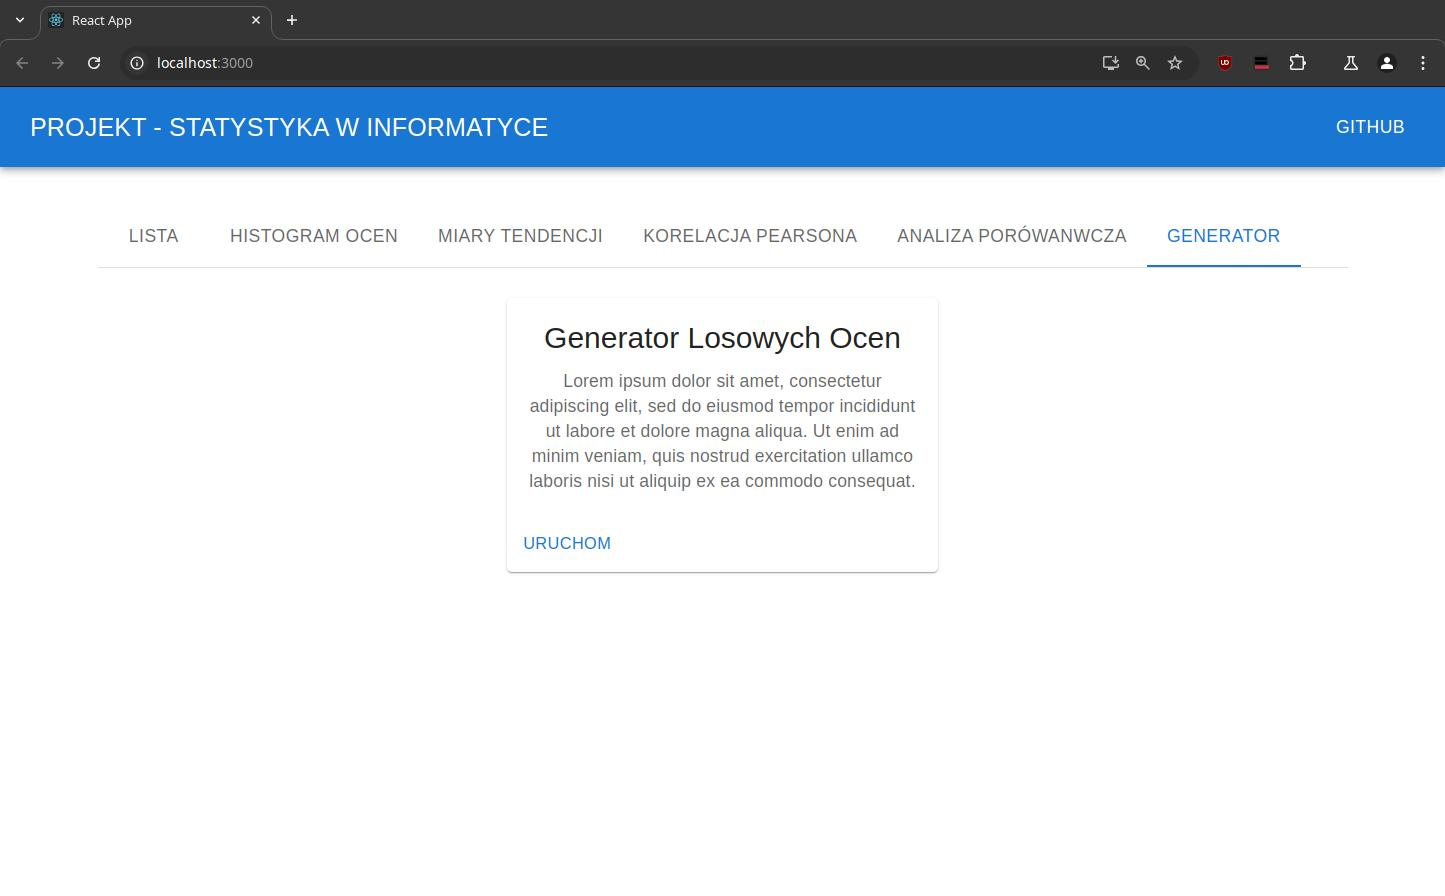
\includegraphics[width=1.0\textwidth]{materiały/generator}
	\caption{Karta generatora}
\end{figure}

\subsection{Generator ocen}
\paragraph{} Generator ocen w projekcie został zaprojektowany z myślą o zapewnieniu różnorodności wyników, co miało na celu odwzorowanie realistycznych scenariuszy oceniania studentów. Proces generowania ocen polega na tworzeniu losowych wyników dla 30 studentów, z uwzględnieniem specyficznych reguł dotyczących każdego przedmiotu, co wpływa na dystrybucję ocen w taki sposób, by były one zróżnicowane, ale jednocześnie sensowne.

Generator działa w następujący sposób:
\begin{enumerate}
	\item \textbf{Wstępne przygotowanie:} Na początku każdorazowo czyszczona jest baza danych, aby móc wygenerować nową pulę ocen.
	\item \textbf{Generowanie ocen:} Dla każdego studenta (30 studentów w projekcie) przypisywane są oceny z 6 przedmiotów. Oceny generowane są losowo, z uwzględnieniem reguł zależnych od przedmiotu:
	\begin{itemize}
		\item \textbf{Informatyka:} Jeśli wylosowana ocena jest wyższa niż 4.0, ale spełniony jest warunek prawdopodobieństwa, ocena jest zmniejszana o 2 punkty.
		\item \textbf{Język obcy:} Na tym przedmiocie wprowadzone są reguły, które preferują ocenę 5.0 lub 4.5 z większym prawdopodobieństwem, a dla niższych ocen ocena jest ustalana w sposób losowy.
		\item \textbf{Fizyka:} Wartość oceny zależy od oceny z matematyki – może być taka sama, lub różnić się o niewielką wartość, jeżeli matematyka jest w średnim zakresie ocen.
		\item \textbf{Matematyka:} Ocena z matematyki jest zapisywana, a potem wykorzystywana do wpływania na inne oceny (np. z fizyki).
		\item \textbf{Wychowanie fizyczne (WF):} Oceny są poprawiane z minimalnej wartości (2.0) na 3.0, aby zapobiec zbyt niskim wynikom.
	\end{itemize}
	\item \textbf{Zapis do bazy:} Po wygenerowaniu oceny dla każdego przedmiotu, dane są dodawane do bazy danych, przechowując informacje o studencie, przedmiocie, ocenie i płci studenta.
\end{enumerate}


W JavaScriptie generowanie liczb losowych odbywa się przy użyciu funkcji \\ \textbf{Math.random()}. Ta funkcja zwraca pseudolosową liczbę zmiennoprzecinkową w przedziale od 0 (włącznie) do 1 (wyłącznie). Wykorzystując tę funkcję, można łatwo generować liczby w dowolnym przedziale, przekształcając wynik \textbf{Math.random()} do pożądanej skali.

\begin{empty}
	\begin{minted}[
		startinline,
		linenos,
		frame=lines,
		framesep=2mm,
		baselinestretch=1.2,
		fontsize=\footnotesize,
		breaklines,
		obeytabs=true,
		tabsize=2,
		]{js}
async function generateMarks ()
{
	db.oceny.clear()
	
	for (let i = 0; i < 30; i++) {
		const [isMan, student] = getRandomName();
		let matma = 2.0;
		
		for (const przedmiot of _przedmioty) {
			let losowaOcena = getRandomOcena();
			
			
			if (przedmiot == "Informatyka" && losowaOcena >= 4.0 && Math.random() < 0.8) {
				losowaOcena -= 2.0;
			}
			
			if (przedmiot == "Język obcy" && Math.random() < 0.3) {
				losowaOcena = Math.random() < 0.5 ? 5.0 : 4.5;
			}
			
			if (przedmiot == "Język obcy" && losowaOcena <= 3.0 && Math.random() < 0.5) {
				losowaOcena = 4.0;
			}
			
			if (przedmiot == "Fizyka") {
				if (Math.random() < 0.5) {
					losowaOcena = matma;
				} else {
					if (matma > 3.0 && matma < 5.0) {
						losowaOcena = matma + (Math.random() < 0.5 ? -0.5 : 0.5);
					}
				}
			}
			
			if (losowaOcena == 2.5) {
				if (Math.random() < 0.5) {
					losowaOcena -= 0.5;
				} else {
					losowaOcena += 0.5;
				}
			}
			
			if (przedmiot == "Matematyka") {
				matma = losowaOcena;
			}
			
			if (przedmiot == "WF" && losowaOcena == 2.0) {
				losowaOcena = 3.0;
			}
			
			const ocena = {
				student: `${student}`,
				przedmiot: przedmiot,
				ocena: losowaOcena,
				plec: isMan
			}
			
			await db.oceny.add(ocena);
		}
	}
}
		
	\end{minted}
	\vspace{-10pt}
	\captionof{listing}{Kod generatora ocen}
\end{empty}

\subsection{Lista studentów}
Wyniki generatora przedstawiamy w tradycyjny sposób - w tabeli, gdzie umieszczone są oceny każdego studenta z poszczególnych przedmiotów.

\begin{figure}[ht]
	\centering
	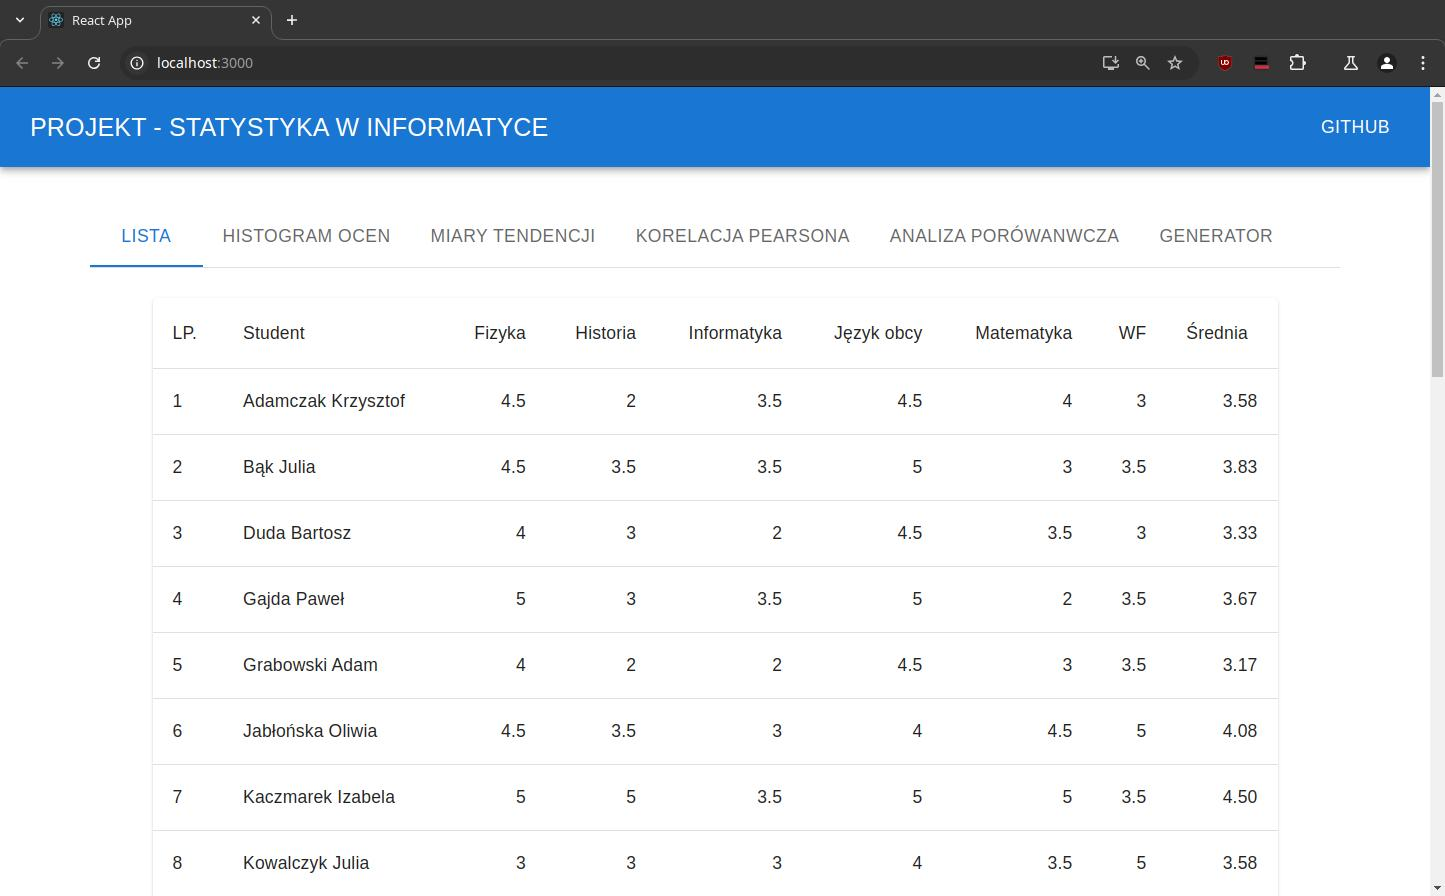
\includegraphics[width=1.0\textwidth]{materiały/lista}
	\caption{Lista studentów wraz z ich ocenami}
\end{figure}

\newpage
\begin{empty}
	\begin{minted}[
		startinline,
		linenos,
		frame=lines,
		framesep=2mm,
		baselinestretch=1.2,
		fontsize=\footnotesize,
		breaklines,
		obeytabs=true,
		tabsize=2,
		]{js}
		async function fetchOceny() 
		{
			await db.oceny; // preload
			const allPrzedmioty = await db.oceny.orderBy('przedmiot').uniqueKeys();//.sort();
			
			const sortedPrzedmioty = allPrzedmioty.sort();
			setPrzedmioty(sortedPrzedmioty);
			
			const dane = [];
			const studenci = await db.oceny.orderBy('student').uniqueKeys();
			const sortedStudenci = studenci.sort();
			
			/** Pobieramy oceny studenta */
			for (const student of sortedStudenci) {
				const ocenyForStudent = await db.oceny
				.where("student")
				.equals(student)
				.sortBy("przedmiot");
				
				dane.push({
					student: student,
					oceny: ocenyForStudent.map(n => n.ocena)
				});
			}
			
			console.log(dane);
			setOceny(dane);
		}
		
	\end{minted}
	\vspace{-10pt}
	\captionof{listing}{Utworzenie obiektu do renderowania w tabelce}
\end{empty}


\subsection{Histogram ocen}
Histogram ocen jest jednym z podstawowych narzędzi wizualizacyjnych w analizie danych, umożliwiającym przejrzyste przedstawienie rozkładu wyników uzyskanych przez studentów z różnych przedmiotów. W projekcie histogram ukazuje, ile razy każda ocena pojawia się w zbiorze danych dla poszczególnych przedmiotów, co pozwala na intuicyjne zrozumienie rozkładu ocen w analizowanej grupie.
\newpage
\begin{figure}[ht]
	\centering
	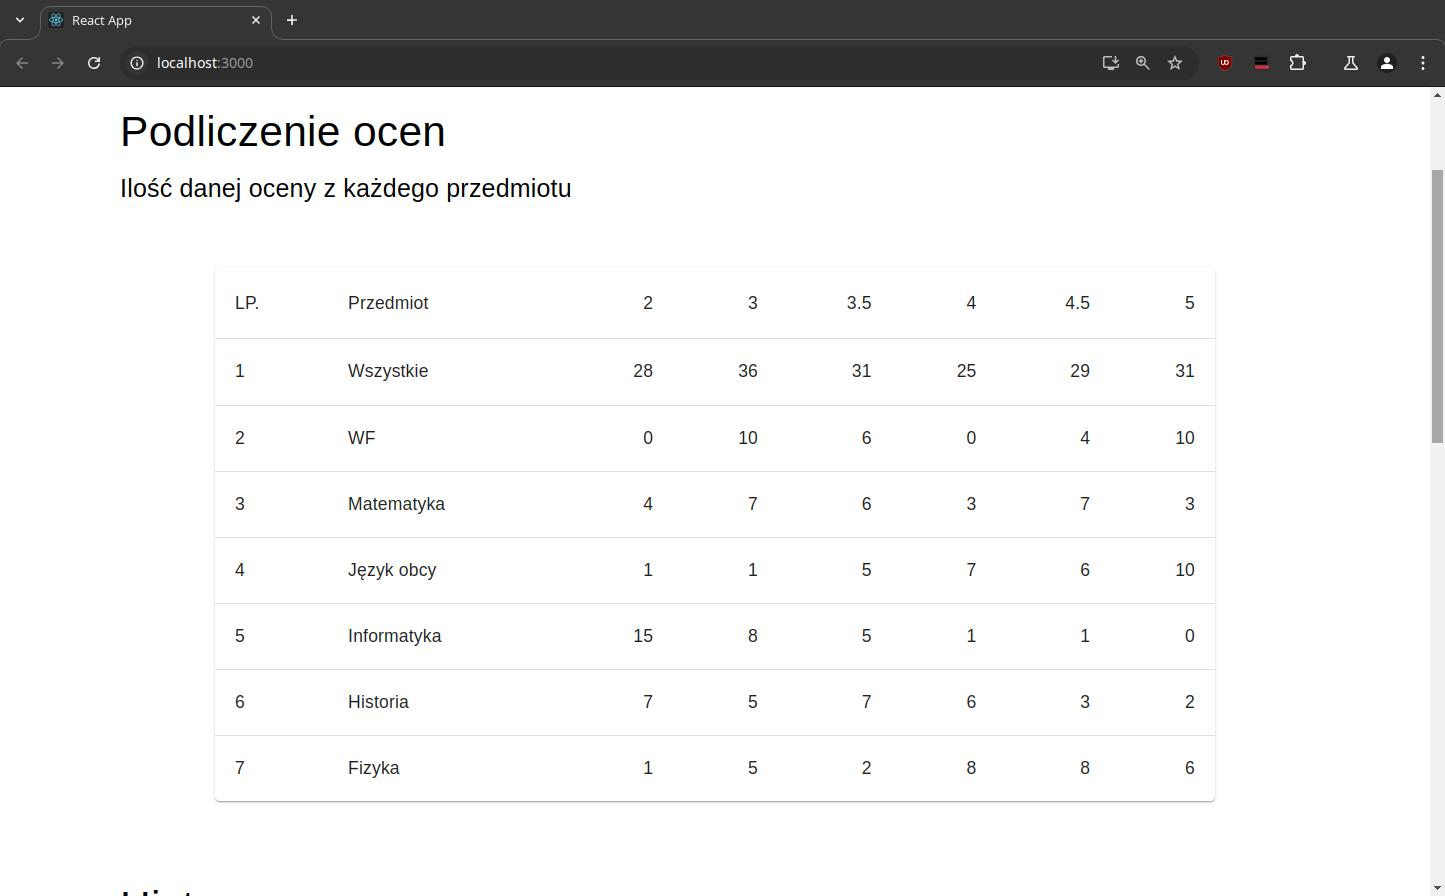
\includegraphics[width=1.0\textwidth]{materiały/histogram1}
	\caption{Tabela podsumowująca ilości ocen}
\end{figure}

\begin{empty}
	\begin{minted}[
		startinline,
		linenos,
		frame=lines,
		framesep=2mm,
		baselinestretch=1.2,
		fontsize=\footnotesize,
		breaklines,
		obeytabs=true,
		tabsize=2,
		]{js}
 const ocenyToHistogram = function (oceny)
{
	const hist = {};
	for (let i = 2.0; i <= 5.0; i+= 0.5) {
		if (i == 2.5) {
			continue;
		}
		hist[`o${i}`] = 0;
	}
	
	for (const ocena of oceny) {
		hist[`o${ocena}`] += 1;
	}
	
	return Object.values(hist);
}
		
	\end{minted}
	\vspace{-10pt}
	\captionof{listing}{Funkcja tworząca histogram ze zbioru ocen}
\end{empty}

\begin{figure}[ht]
	\centering
	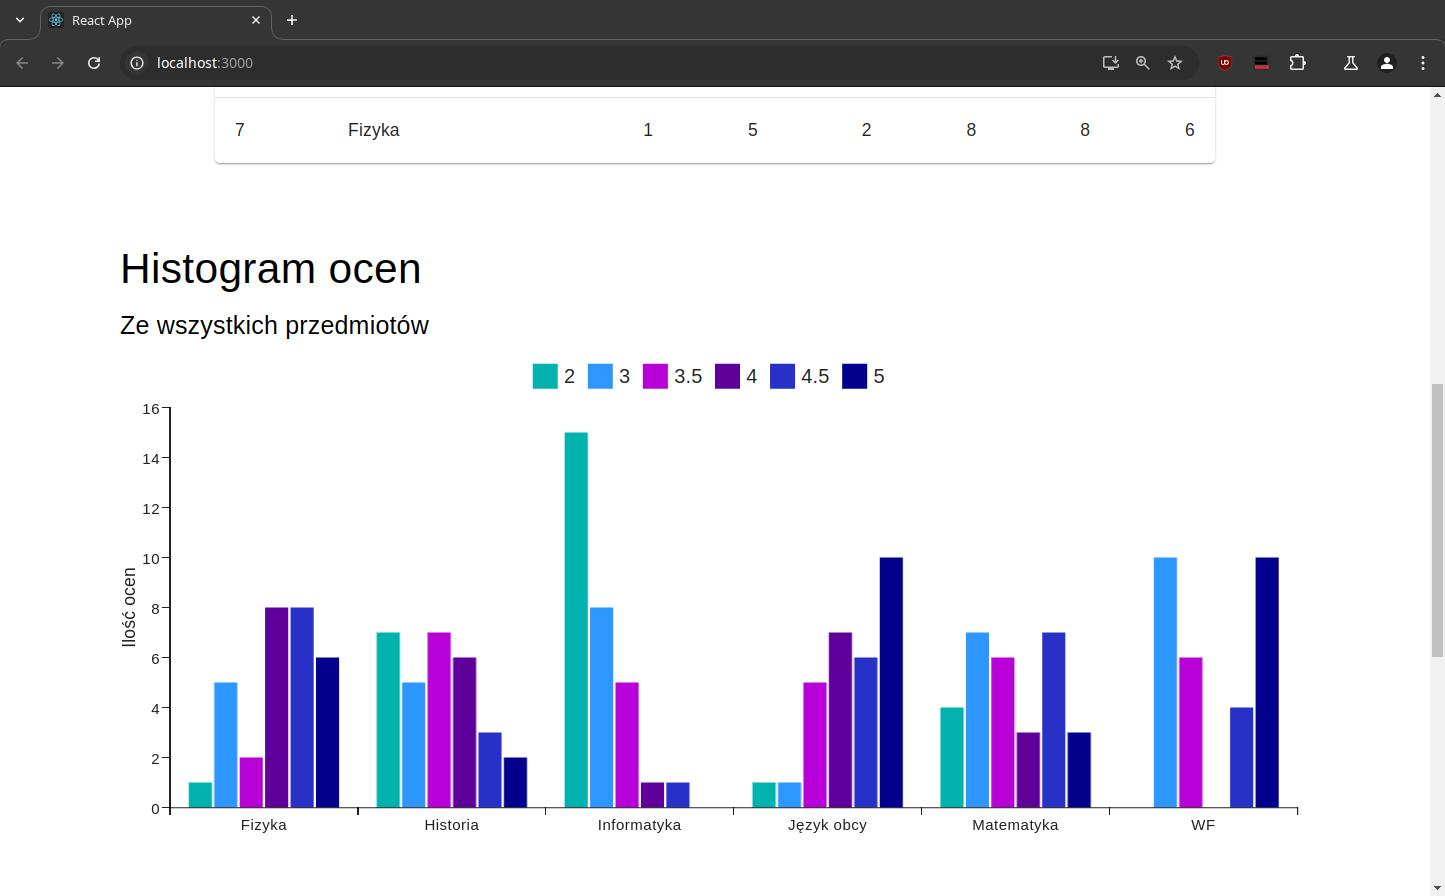
\includegraphics[width=1.0\textwidth]{materiały/histogram2}
	\caption{Histogram ocen}
\end{figure}
\newpage
Dzięki powyższym informacjom, możemy również przeanalizować ogólną ilość poszczególnych stopni. Przedstawimy to na wykresie kołowym:
\begin{figure}[ht]
	\centering
	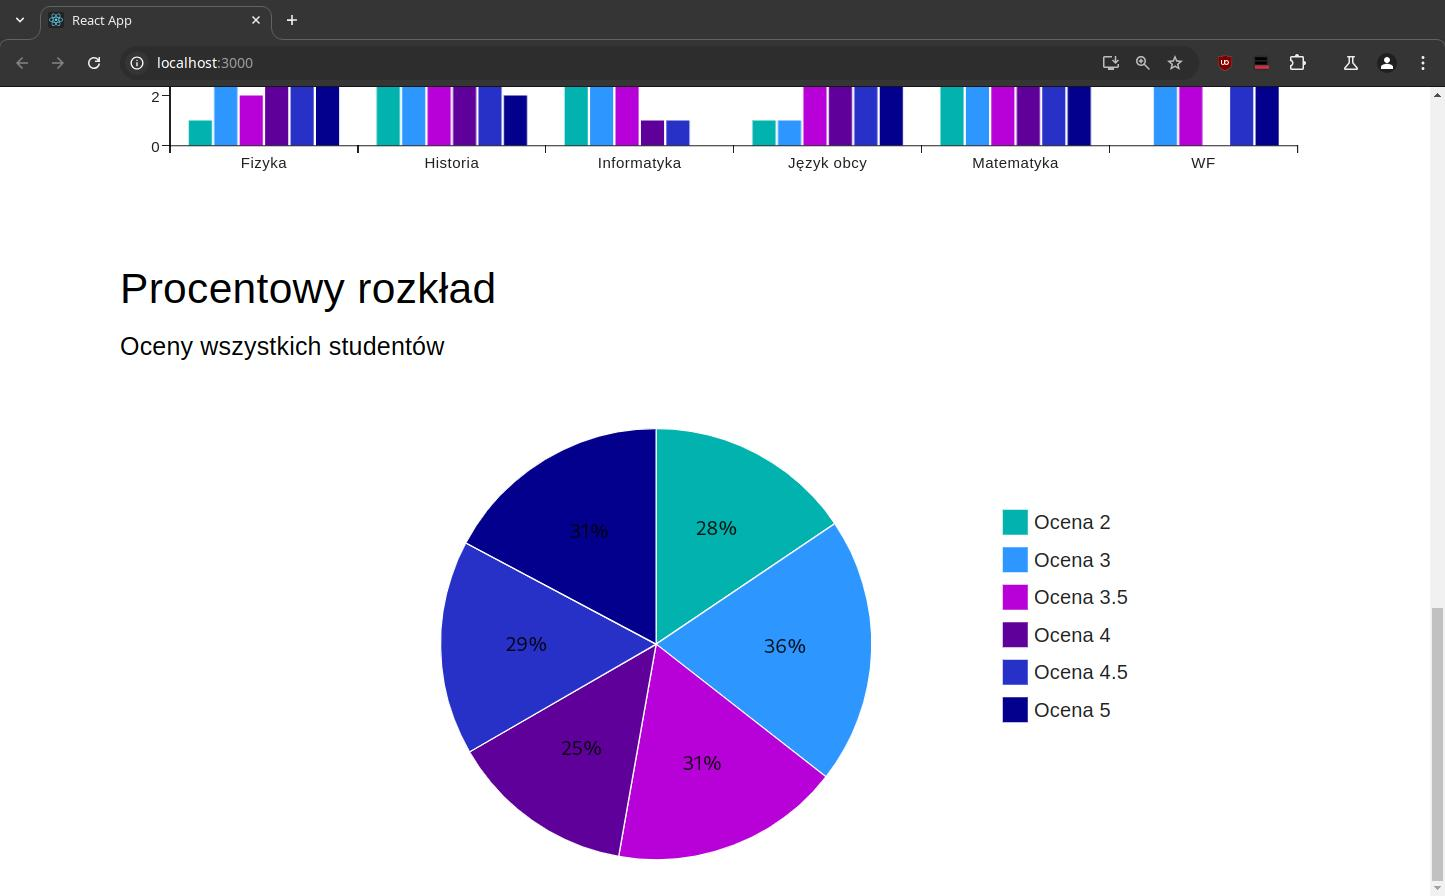
\includegraphics[width=1.0\textwidth]{materiały/histogram3}
	\caption{Histogram ocen}
\end{figure}

\begin{empty}
	\begin{minted}[
		startinline,
		linenos,
		frame=lines,
		framesep=2mm,
		baselinestretch=1.2,
		fontsize=\footnotesize,
		breaklines,
		obeytabs=true,
		tabsize=2,
		]{jsx}
<PieChart 
	width={700}
	height={400}
	series={[{
		arcLabel: (item) => `${item.value}%`,
		arcLabelMinAngle: 35,
		arcLabelRadius: '60%',
		data: histogram.filter(n => n.przedmiot == "Wszystkie").at(0).hist.map((n, i) => {
			return {
				id: i,
				value: n,
				label: `Ocena ${2.0 + i * 0.5 + (i >= 1 ? 0.5 : 0)}`
			}
		})
	}]}
/>
		
	\end{minted}
	\vspace{-10pt}
	\captionof{listing}{Generowanie wykresu kołowego}
\end{empty}

\subsection{Miary tendencji}
Miary tendencji centralnej i zmienności są kluczowymi wskaźnikami w analizie danych statystycznych, pozwalającymi określić podstawowe właściwości rozkładu ocen. W projekcie wyznaczono następujące wskaźniki: średnią arytmetyczną, medianę, dominantę, wariancję oraz odchylenie standardowe. Każda z tych miar dostarcza cennych informacji o danych i pozwala na lepsze zrozumienie wyników studentów.

\begin{itemize}
	\item \textbf{Średnia arytmetyczna}: Średnia arytmetyczna (oznaczana jako \( \bar{X} \)) to suma wszystkich wartości w zbiorze, podzielona przez liczbę tych wartości. Średnia arytmetyczna jest podstawową miarą tendencji centralnej.
	\[
	\bar{X} = \frac{1}{n} \sum_{i=1}^{n} X_i
	\]
	gdzie:
	\begin{itemize}
		\item \( X_i \) – wartość pojedynczej obserwacji,
		\item \( n \) – liczba obserwacji.
	\end{itemize}
	
	\item \textbf{Mediana}: Mediana to środkowa wartość zbioru uporządkowanych danych. W przypadku liczby nieparzystej jest to wartość dokładnie w środku, a przy liczbie parzystej – średnia arytmetyczna dwóch środkowych wartości.
	
	\item \textbf{Dominanta}: Dominanta, czyli wartość modalna, to wartość występująca najczęściej w zbiorze danych. Jest to prosta miara, która pozwala zidentyfikować najczęściej uzyskiwaną ocenę.
	
	\item \textbf{Wariancja}: Wariancja (oznaczana jako \( \sigma^2 \)) jest miarą rozproszenia danych wokół średniej. Oblicza się ją jako średnią kwadratów odchyleń poszczególnych wartości od średniej.
	\[
	\sigma^2 = \frac{1}{n} \sum_{i=1}^{n} (X_i - \bar{X})^2
	\]
	
	\item \textbf{Odchylenie standardowe}: Odchylenie standardowe (\( \sigma \)) to pierwiastek kwadratowy z wariancji. Jest intuicyjną miarą rozproszenia, wyrażoną w tych samych jednostkach co wartości w zbiorze danych.
	\[
	\sigma = \sqrt{\sigma^2} = \sqrt{\frac{1}{n} \sum_{i=1}^{n} (X_i - \bar{X})^2}
	\]
\end{itemize}

Te miary pozwalają uzyskać szczegółowy wgląd w rozkład ocen studentów, w tym średnią wartość wyników, częstość występowania ocen, a także stopień ich zróżnicowania.
\begin{empty}
	\begin{minted}[
		startinline,
		linenos,
		frame=lines,
		framesep=2mm,
		baselinestretch=1.2,
		fontsize=\footnotesize,
		breaklines,
		obeytabs=true,
		tabsize=2,
		]{js}
const getMedian = function (oceny)
{
	const sorted = oceny.sort();
	
	if (sorted % 2 != 0)
		return sorted[parseInt(Math.floor(sorted.length / 2))];
	
	const half = sorted.length / 2;
	return (oceny[half] + oceny[half - 1]) / 2;
}

const getDominion = function (oceny)
{
	const counts = {};
	for (let i = 2.0; i <= 5.0; i += 0.5) {
		counts[`o${i}`] = 0;
	}
	
	for (let ocena of oceny) {
		counts[`o${ocena}`] += 1;
	}
	
	const domain = [];
	const most = Object.values(counts).reduce((a, b) => Math.max(a, b));
	for (const [k, v] of Object.entries(counts)) {
		if (v == most) {
			domain.push(k.substring(1));
		}
	}
	
	return domain.join(", ");
}

const prepMeasures = function (oceny)
{
	const res = [];
	const avg = oceny.reduce((a, b) => a + b) / oceny.length;
	res.push(avg.toFixed(2));
	res.push(getMedian(oceny).toFixed(2));
	res.push(getDominion(oceny));
	
	const war = oceny.map(n => Math.pow(n - avg, 2)).reduce((a, b) => a + b) / oceny.length;
	res.push(war.toFixed(2));
	res.push(Math.sqrt(war).toFixed(2));
	
	return res;
}	
	\end{minted}
	\vspace{-10pt}
	\captionof{listing}{Programistyczne podejście do matematycznych obliczeń}
\end{empty}

\begin{figure}[ht]
	\centering
	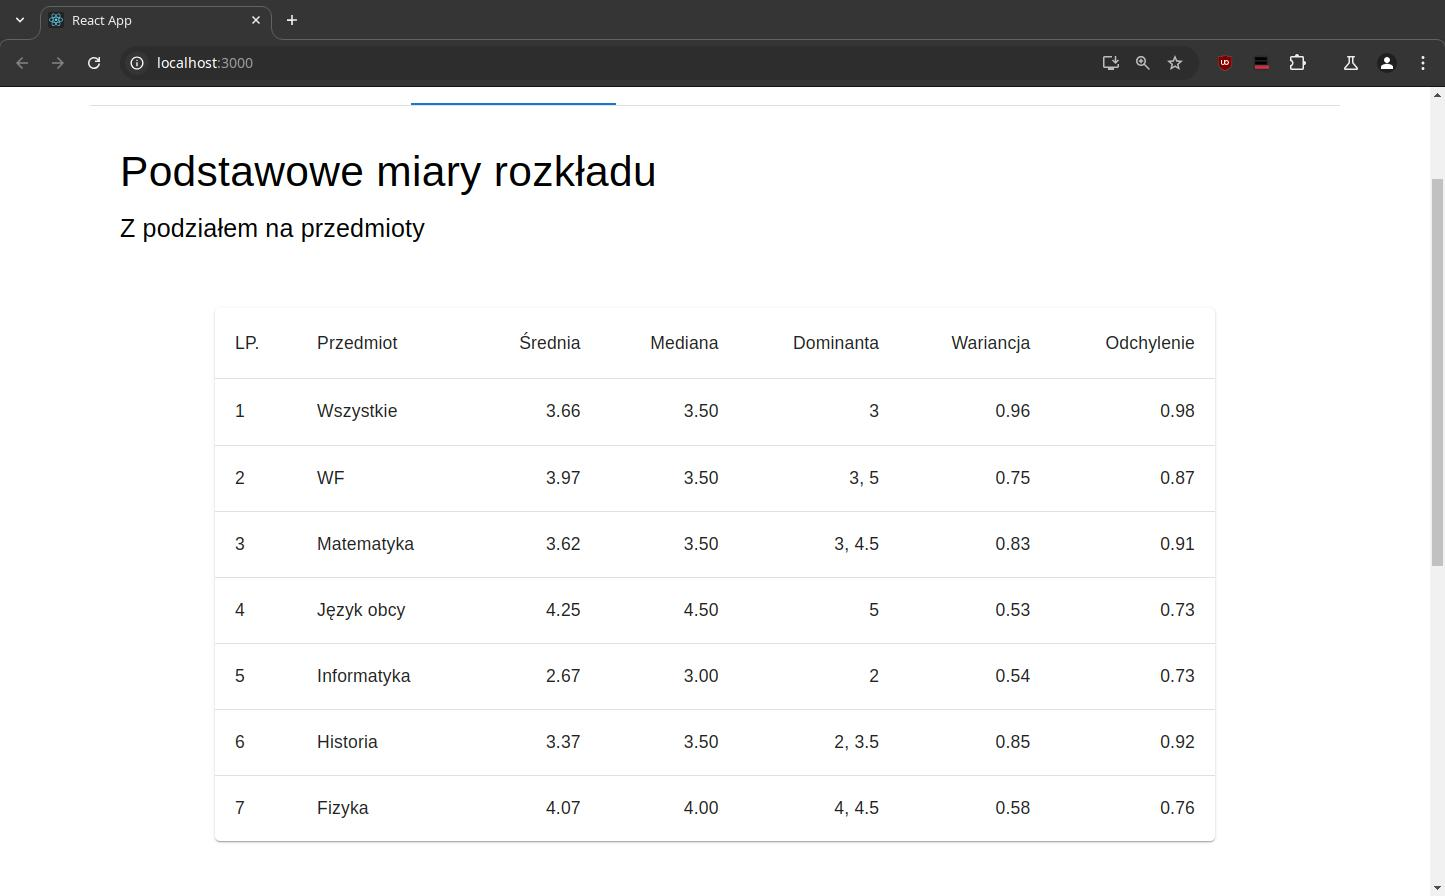
\includegraphics[width=1.0\textwidth]{materiały/miary}
	\caption{Tabela podsumowująca wyniki}
\end{figure}

\subsection{Korelacja Pearsona}
Współczynnik korelacji Pearsona jest miarą liniowej zależności pomiędzy dwiema zmiennymi. Wartość współczynnika korelacji przyjmuje wartości od \( -1 \) do \( 1 \). Współczynnik ten pozwala ocenić, czy wzrost jednej zmiennej wiąże się ze wzrostem lub spadkiem drugiej zmiennej oraz w jakim stopniu. Interpretacja współczynnika korelacji jest następująca:
\begin{itemize}
	\item Wartość \( r = 1 \) oznacza doskonałą dodatnią korelację liniową.
	\item Wartość \( r = -1 \) oznacza doskonałą ujemną korelację liniową.
	\item Wartość \( r = 0 \) wskazuje na brak korelacji liniowej między zmiennymi.
\end{itemize}

Współczynnik korelacji Pearsona \( r \) jest obliczany według wzoru:
\[
r = \frac{\sum_{i=1}^{n} (X_i - \bar{X})(Y_i - \bar{Y})}{\sqrt{\sum_{i=1}^{n} (X_i - \bar{X})^2} \cdot \sqrt{\sum_{i=1}^{n} (Y_i - \bar{Y})^2}}
\]
gdzie:
\begin{itemize}
	\item \( X_i \) i \( Y_i \) – wartości dwóch zmiennych dla \( i \)-tego przypadku,
	\item \( \bar{X} \) i \( \bar{Y} \) – średnie arytmetyczne zmiennych \( X \) i \( Y \),
	\item \( n \) – liczba obserwacji.
\end{itemize}

Wartość współczynnika korelacji Pearsona w analizie danych z ocenami pozwala na identyfikację zależności między wynikami z różnych przedmiotów. Dzięki temu można określić, czy istnieje statystycznie istotna zależność pomiędzy ocenami z dwóch różnych przedmiotów, co może pomóc w zrozumieniu, czy osiągnięcia w jednym przedmiocie mają tendencję do wzrostu lub spadku wraz z wynikami w innym.

\begin{figure}[ht]
	\centering
	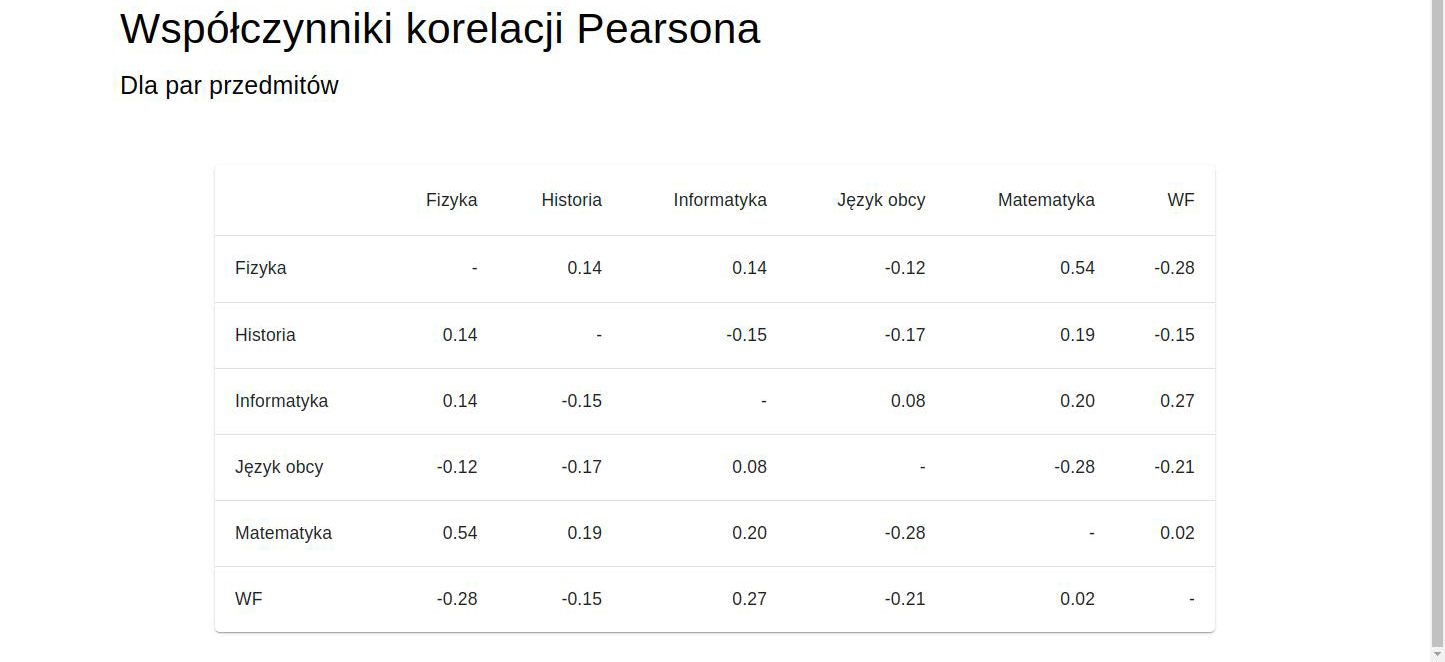
\includegraphics[width=1.0\textwidth]{materiały/korelacja}
	\caption{Tabela podsumowująca wyniki}
\end{figure}

\subsection{Analiza porównawcza}
Aplikacja umożliwia porównanie zdawalności z poszczególnych przedmiotów z podziałem na płeć studenta.

\begin{figure}[ht]
	\centering
	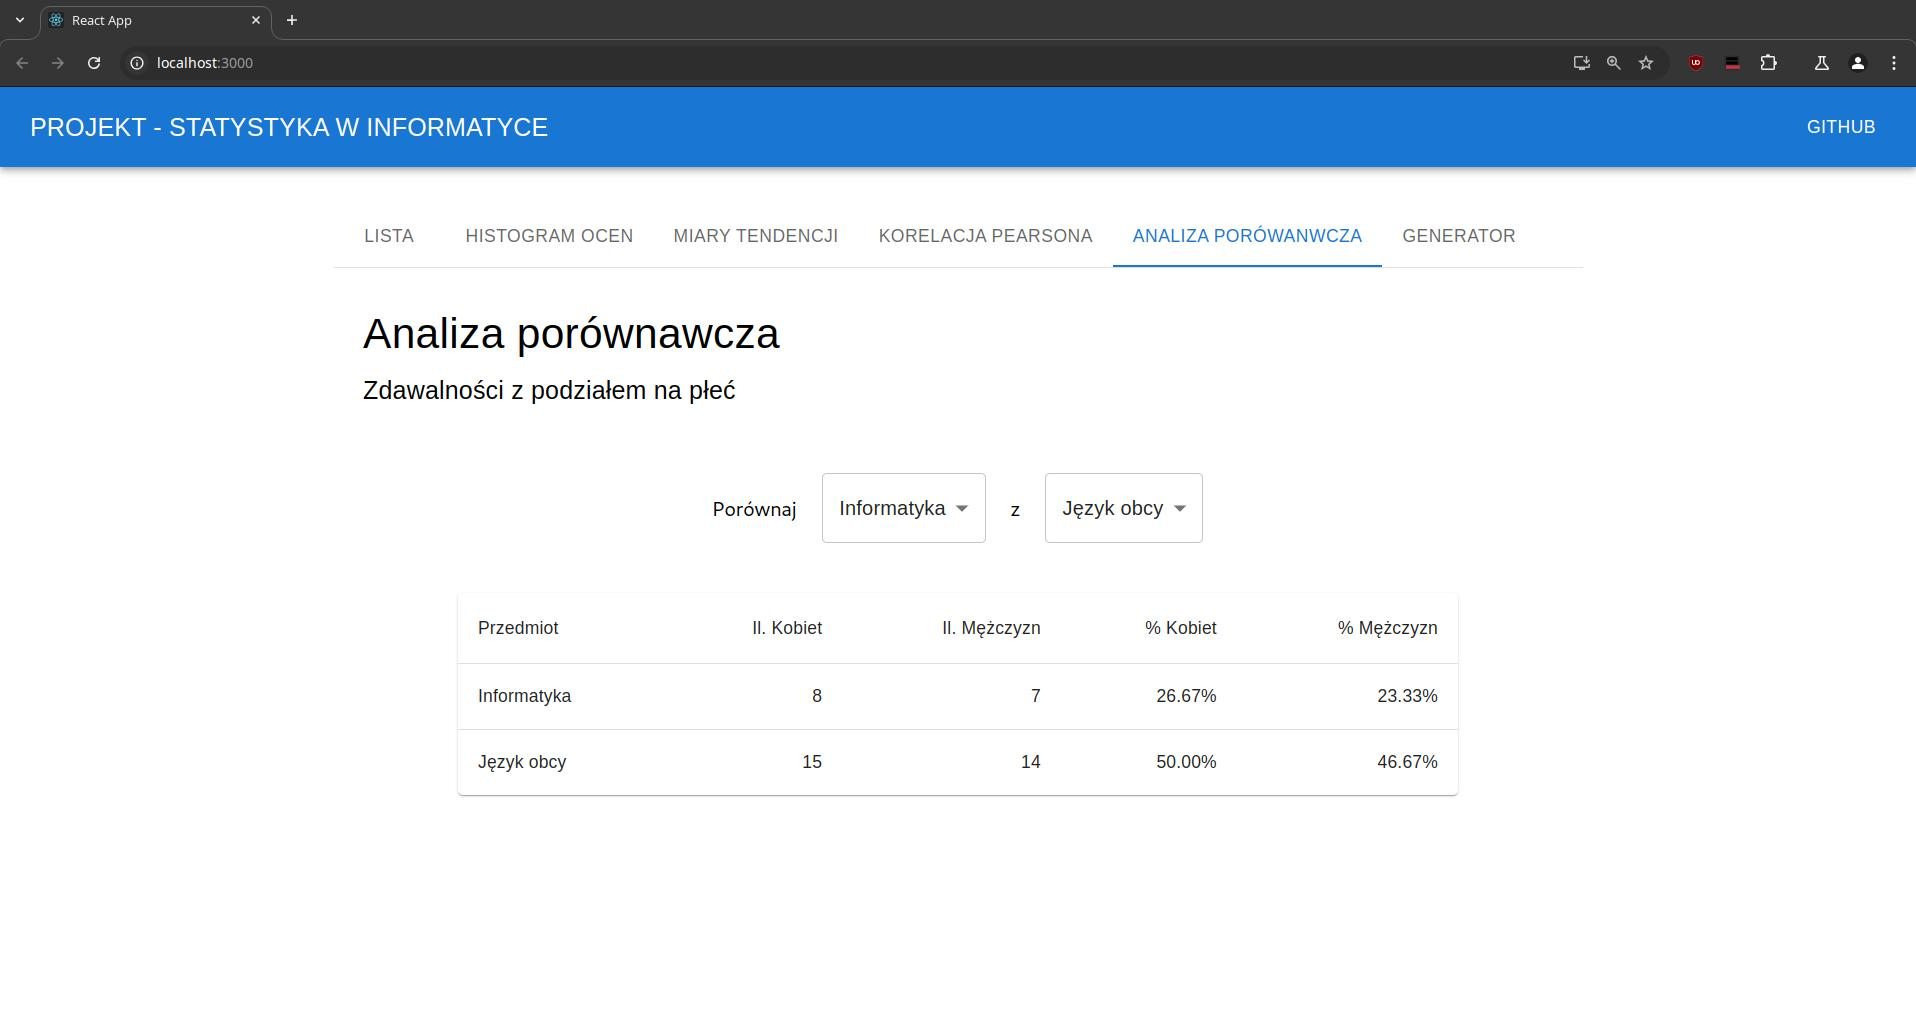
\includegraphics[width=1.0\textwidth]{materiały/analiza}
	\caption{Tabela podsumowująca wyniki}
\end{figure}

\section{Instrukcja uruchomienia aplikacji}

Aby uruchomić aplikację stworzoną w React, należy wykonać kilka kroków konfiguracyjnych:

\begin{enumerate}
	\item \textbf{Zainstaluj Node.js i npm} \\
	Upewnij się, że na komputerze zainstalowane są \textbf{Node.js} oraz \textbf{npm} (Node Package Manager). Node.js jest niezbędny do uruchamiania aplikacji w React, a npm służy do zarządzania bibliotekami.
	
	Aby sprawdzić, czy są zainstalowane, uruchom następujące polecenia w terminalu:
	\begin{verbatim}
		node -v
		npm -v
	\end{verbatim}
	Jeśli nie masz ich zainstalowanych, pobierz odpowiednie wersje z \url{https://nodejs.org/}.
	
	\item \textbf{Sklonuj repozytorium z kodem aplikacji} \\
	Kod znajduje się w repozytorium na GitHubie, sklonuj go lokalnie za pomocą polecenia:
	\begin{verbatim}
		git clone https://github.com/quakcin/Statystyka-w-informatyce-Projekt
	\end{verbatim}
	Następnie przejdź do katalogu projektu:
	\begin{verbatim}
		cd Statystyka-w-informatyce-Projekt/uusos
	\end{verbatim}
	
	\item \textbf{Zainstaluj zależności} \\
	W katalogu projektu uruchom następujące polecenie, aby zainstalować wszystkie wymagane biblioteki:
	\begin{verbatim}
		npm install
	\end{verbatim}
	
	\item \textbf{Uruchom aplikację w trybie deweloperskim} \\
	Po zakończeniu instalacji zależności uruchom aplikację w trybie deweloperskim za pomocą komendy:
	\begin{verbatim}
		npm start
	\end{verbatim}
	Aplikacja zostanie uruchomiona, a domyślnie będzie dostępna pod adresem \url{http://localhost:3000}. Po wprowadzeniu zmian w kodzie aplikacja automatycznie się przeładuje.
\end{enumerate}

\section{Podsumowanie}
W ramach projektu "Analiza wyników egzaminów studentów z różnych przedmiotów" zaprezentowano narzędzie do analizy i wizualizacji ocen studentów. Aplikacja została oparta na bibliotece React, a dane o ocenach studentów były generowane przy pomocy autorskiego generatora, co pozwoliło na uzyskanie różnorodności ocen. Wszystkie dane zostały przechowywane w bazie Dexie.js, która zapewniała wygodny dostęp do danych bez potrzeby implementacji backendu.

W projekcie zostały obliczone podstawowe miary statystyczne, takie jak średnia, mediana, dominanta, wariancja, odchylenie standardowe oraz współczynnik korelacji Pearsona. Te miary umożliwiają analizę rozkładu wyników w poszczególnych przedmiotach oraz między przedmiotami, dostarczając cennych informacji o osiągnięciach studentów.

Aplikacja umożliwia także wizualizację danych za pomocą wykresów, w tym histogramu ocen, co pozwala na łatwe zrozumienie rozkładu wyników. Interfejs aplikacji jest przyjazny dla użytkownika, dzięki zastosowaniu biblioteki MUI.

Projekt umożliwia przeprowadzenie szczegółowej analizy wyników studentów. Dzięki elastyczności aplikacji, możliwe jest dostosowanie jej do różnych wymagań analitycznych i rozwoju w przyszłości.
